\documentclass[letterpaper]{article} 
\usepackage[left = 0.5in, right = 0.5in, top = 0.9in, bottom = 0.9in]{geometry}
\usepackage{enumitem}
\usepackage{multicol}
\usepackage[spanish]{babel}
\usepackage[utf8]{inputenc}

\usepackage{amsmath,amssymb,amsthm}
\usepackage{tikz-cd}
\usepackage{mathrsfs}
\usepackage[bbgreekl]{mathbbol}
\usepackage{dsfont}
\usepackage{listings}
\usepackage{graphicx}
\graphicspath{{img/}}
\newcommand{\op}{\operatorname}
\newcommand{\Op}{^{\op{op}}}
\newcommand{\scc}{\mathscr C}
\newcommand{\scd}{\mathscr D}
\newcommand{\sce}{\mathscr E}
\newcommand{\sci}{\mathscr I}
\newcommand{\scj}{\mathscr J}
\newcommand{\scx}{\mathscr X}
\newcommand{\var}{\mathrm{Var}}
\newcommand{\Id}{\operatorname{Id}}
\newcommand{\N}{\mathbb N}
\newcommand{\Z}{\mathbb Z}
\newcommand{\Q}{\mathbb{Q}}
\newcommand{\I}{\mathbb{I}}
\newcommand{\R}{\mathbb{R}}
\newcommand{\C}{\mathbb{C}}
\newcommand{\F}{\mathcal{F}}
\newcommand{\G}{\mathcal{G}}
\newcommand{\abs}[1]{\left\lvert #1 \right\rvert}
\newcommand{\inv}{^{-1}}
\renewcommand{\to}{\longrightarrow}
\newcommand{\ent}{\Longrightarrow}
\newcommand{\E}{\mathbb{E}}
\renewcommand{\P}{\mathbb{P}}
\newcommand{\1}{\mathds{1}}

\theoremstyle{definition}
\newtheorem{dfn}{Definición}
\theoremstyle{definition}
\newtheorem{teo}{Teorema}
\theoremstyle{definition}
\newtheorem{cor}{Corolario}
\theoremstyle{definition}
\newtheorem{prop}{Proposición}
\theoremstyle{definition}
\newtheorem{obs}{Observación}


\title{\textbf{Cómputo Científico\\
Tarea 1\\
Descomposición LU y Cholesky}}
\author{Iván Irving Rosas Domínguez}
\date{\today}

\DeclareSymbolFontAlphabet{\mathbbm}{bbold}
\DeclareSymbolFontAlphabet{\mathbb}{AMSb}
\DeclareMathSymbol\bbDelta  \mathord{bbold}{"01}

\begin{document}
\maketitle

% \begin{abstract}
% \end{abstract}

\begin{enumerate}
    \item Implementar los algoritmos de \textit{Backward y Forward substitution}.\\
    
    \textbf{Solución:} La implementación de los algoritmos anteriores se
     puede apreciar en el script 'Algoritmos'. Las funciones de los respectivos
     algoritmos son llamadas a través de los nombres $forsub(M,a)$ y $backsub(M,a)$,
     donde $M$ y $a$ son las respectivas matrices y vectores que forman los
     sistemas triangulares que los algoritmos van a resolver. Los comentarios sobre
     el funcionamiento del algoritmo se encuentran en este archivo.

    \item Implementar el algoritmo de eliminación gaussiana con pivoteo parcial LUP,
    21.1 del Trefethen (p.160).\\

    \textbf{Solución:} La implementación de este algoritmo se aprecia nuevamente en
    el script 'Algoritmos'. La función que implementa dicho algoritmo tiene el nombre
    de $LUPfact(A)$, donde $A$ es la matriz a descomponer. También se encuentran aquí
    los comentarios sobre el funcionamiento del algoritmo.

    \item Dar la descomposición LUP para una matriz aleatoria de entradas $U(0,1)$
    de tamaño $5\times5$, y para la matriz
    \[
        A=
        \begin{pmatrix}
          1 & 0 & 0 & 0 & 1\\
         -1 & 1 & 0 & 0 & 1\\
         -1 & -1 & 1 & 0 & 1\\
         -1 & -1 & -1 & 1 & 1\\
         -1 & -1 & -1 & -1 & 1\\
        \end{pmatrix}
    \]
    \textbf{Solución:} Este ejercicio se encuentra realizado en la primera parte del script 'Ejercicio 2-3'.
    En tal script se detalla el funcionamiento del código en sí de ambos ejercicios\\

    Para la solución de estos ejercicios, se cargan primero las librerías a utilizar,
    que son $numpy$ y de la librería $scipy.stats$ se importa $uniform$.
    También se cargan las funciones a utilizar, a saber, las funciones $LUPfact$, 
    $backsub$ y $forsub$, de los respectivos algoritmos que implementan.
    \newline
    \begin{itemize}
    \item Lo primero que se realiza en el script es la descomposición LUP de una matriz con
    entradas aleatorias uniformes en $(0,1)$ y de tamaño $5\times5$. Para ello, y con
    la finalidad de poder repetir el experimento, se coloca primero
    una semilla para generar los números aleatorios. La elección de la semilla $n$ es
    $n=10$.\\

    Generada la semilla, procedemos a extraer una muestra aleatoria de tamaño 25
    de la distribución uniforme en $(0,1)$, las cuales se guardan en un vector $M$
    de tamaño 25, y posteriormente se reorganiza dicho vector en un arreglo 
    2-dimensional de $numpy$, obteniendo así la matriz buscada. Se presenta en el script la
    posibilidad de visualizar de antemano dicha matriz generada.\\

    Posteriormente se realiza la descomposición LUP aplicando la función $LUPfact$ 
    a nuestra matriz $M$. En el paso anterior, se extraen las matrices
    que la función $LUPfact(M)$ genera (ver comentarios respectivos del script 'Algoritmos'),
    para una visualización lo más cercana posible a la forma 
    \[
    PA=LU    
    \]
    de la descomposición, donde $PM$ es la matriz de permutación, $A$ es la matriz original
    (en este caso $A=M$) y $LM, UM$ son las matrices triangulares inferiores y superiores
    respectivamente que descomponen el producto de la izquierda. Obtenemos así la siguiente
    descomposición: 
    \begin{figure}[h]
        \centering
        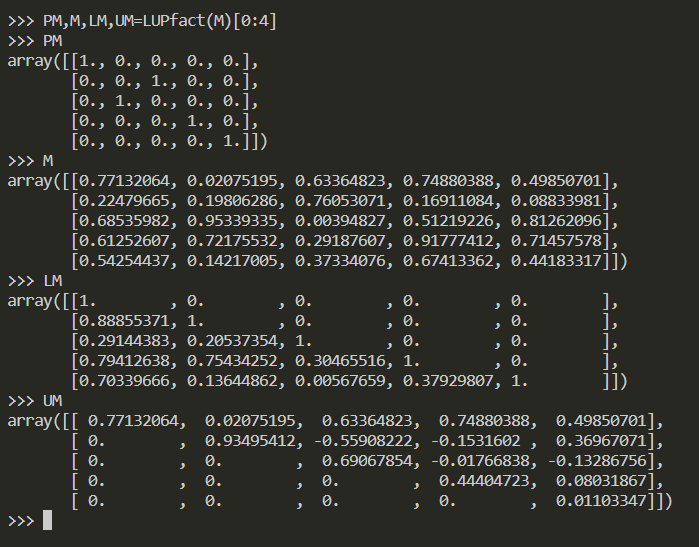
\includegraphics[width=0.5\linewidth]{a.png}
        \caption[Figura 1]{Descomposición LUP de la matriz aleatoria M.}
    \end{figure}
    \item Para el segundo ejemplo en donde se debe descomponer la matriz A dada al inicio
    de este ejercicio, procedemos simplemente ejecutando el algoritmo LUP en 
    la consola para obtener la factorización. Nuevamente obtenemos las matrices de tal
    forma que recuperemos lo más posible la forma $PA=LU$. El resultado se muestra a continuación:
    \begin{figure}[h]
        \centering
        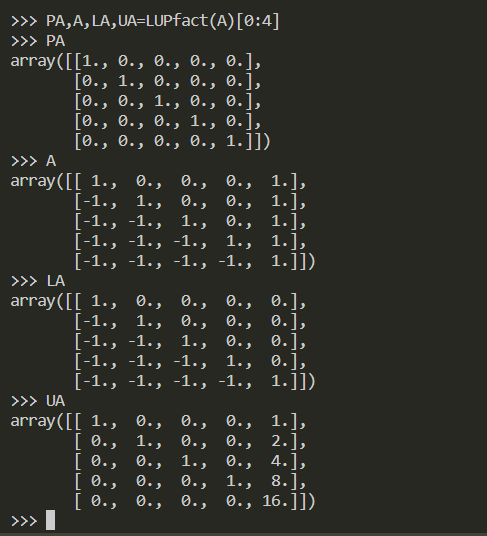
\includegraphics[width=0.3\linewidth]{b.png}
        \caption[Figura 2]{Descomposición LUP de la matriz A anterior.}
    \end{figure}
    \end{itemize}
    \item Usando la descomposición LUP anterior, resolver el sistema de la forma
    \[
    Dx=b    
    \]
    donde $D$ son las matrices del problema 3, para 5 diferentes $b$ aleatorios
    con entradas $U(0,1)$. Verificando si es o no posible resolver el sistema.\\

    \textbf{Solución:} Como se comentó en el ejercicio anterior, este ejercicio tiene
    el código implementado en el script 'Ejercicios 3-4'. Ya con las matrices $M$ y $A$
    del ejercicio anterior, generamos cinco vectores aleatorios $b$ para resolver los
    sistemas de ecuaciones $Mx=b$ y $Ax=b$.\\

    Para ello, como antes, sembramos una semilla para poder replicar los resultados.
    En este caso elegimos $n=5$. Creamos un arreglo de tamaño 25 con los números aleatorios
    uniformes en $(0,1)$ y posteriormente formamos una matriz $B$ de tamaño $5\times5$.
    Pensaremos en cada columna de la matriz $B$ como los respectivos 5 vectores $b$ aleatorios.\\

    Con los vectores $b$ y las matrices $M$ y $A$ cargadas, junto con sus respectivas 
    factorizaciones ya hechas, procedemos a implementar los algoritmos $backward$ y
    $forward$, recordando que usando una matriz $R$ y factorizándola con LU, 
    \[
    Rx=b \ \text{y} \ PR=LU \ \ent \ LUx=Pb,    
    \]
    de tal forma que, haciendo $Ux=y$, tenemos que resolver los sistemas
    \[
        Ly=Pb \ \text{y} \ Ux=y,
    \]
    en ese orden, para obtener el vector $x$ que sea solución del sistema $Rx=b$. 
    
    \begin{itemize}
    \item   Procedemos pues a solucionar los sistemas de ecuaciones para la matriz $M$ primero,
    para cada uno de los cinco vectores $b$ aleatorios. El resultado lo guardamos en una nueva matriz que llamamos
    $XM$ ($XA$ para la la matriz $A$), cuyos vectores columna sean los resultados de las soluciones de los 5 sistemas
    de ecuaciones. La razón de lo anterior es que podemos verificar si
    el sistema de ecuaciones en efecto fue resuelto simplemente realizando el producto de las
    matrices $M,XM$ y verificando si en efecto dicho producto coincide con la matriz $B$.
    \newline

    Realizando lo anterior, obtenemos que en efecto el producto coincide, tal y como se muestra.
    \begin{figure}[h]
        \centering
        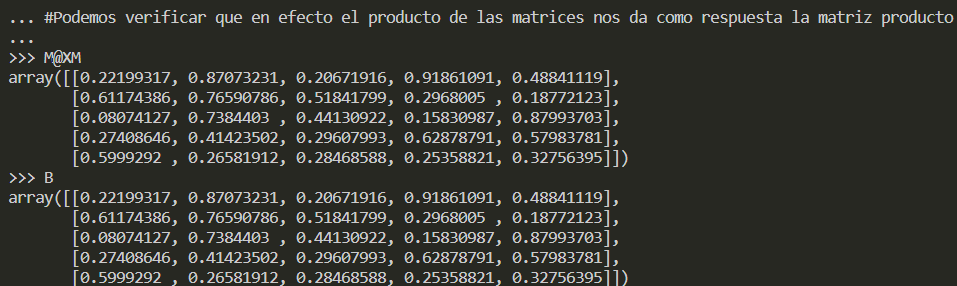
\includegraphics[width=0.5\linewidth]{c.png}
        \caption[Figura 3]{Verificación del producto $M\cdot XM$ con la matriz $B$. Ambos coinciden}
    \end{figure}
    \item Para el segundo ejemplo, replicamos exactamente el mismo procedimiento: colocamos una
    semilla, generamos la matriz $B$ aleatoria (la semilla para este ejemplo es $n=15$), y 
    corremos el script, obteniendo la matriz $XA$ solución, y notamos que el producto de las matrices $A$
     y $XA$, comparado con la matriz $B$, queda de la siguiente forma:
     \begin{figure}[h]
        \centering
        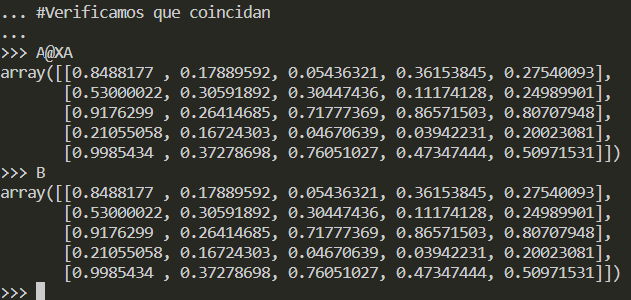
\includegraphics[width=0.5\linewidth]{d.png}
        \caption[Figura 4]{Verificación del producto $A\cdot XA$ con la matriz $B$. Ambos coinciden}
    \end{figure}
\end{itemize}

    \item Implementar el algoritmo de descomposición de Cholesky 23.1 del 
    Trefethen (p.175).\\

    \textbf{Solución:} La implementación de este algoritmo se encuentra nuevamente
    el script 'Algoritmos'. La función que implementa el algoritmo tiene el nombre
    de $CholFact(A)$, donde $A$ es la matriz hermitiana definida positiva
    que se va a descomponer, y los comentarios sobre el funcionamiento de
    este comentario se encuentran en su respectiva sección.\\

    \item Comprara la complejidad de su implementación de los algoritmos de 
    factorización de Cholesky y LUP mediante la medición de los tiempos
    que tardan con respecto a la descomposición de una matriz aleatoria hermitiana
    definida positiva. Graficar la comparación.\\

    \textbf{Solución:} Para este ejercicio, primero cargamos en el script 'Ejercicio 5' todas las paqueterías
     a usar: $numpy, time, scipy$ y $matplotlib$, junto con las funciones de los algoritmos LUP y Cholesky. 
    Luego creamos una sucesión de matrices aleatorias con entradas
    de distribución uniforme en $(0,1)$, y de tamaños entre 1 y 300, con una semilla $n=5$.
    \newline

    Posteriormente creamos matrices hermitianas definidas positivas reacomodando los vectores
    que se crean sucesivamente en arreglos cuadrados, y multiplicándo las matrices resultantes por
    su transpuesta, para que así, tengamos matrices simétricas y definidas positivas.
    \newline

    Creamos vectores de tiempos de ejecución de tamaño 300, uno para cada uno de los algoritmos.
    La idea es que en cada ciclo de ejecución de los algoritmos se mida el tiempo que
    tarda la computadora en ejecutar un algoritmo vs el tamaño de la matriz, y graficar los resultados.
    \\

    Después de realizar tal labor y graficar con la librería $matplotlib$, obtenemos lo siguiente:

    \begin{figure}[h]
        \centering
        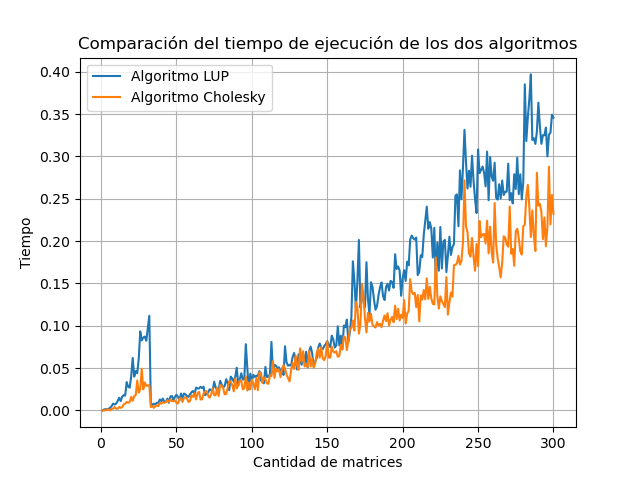
\includegraphics[width=0.5\linewidth]{e.png}
        \caption[Figura 5]{Comparación de los tiempos de ejecución. El algoritmo de Cholesky es más rápido.}
    \end{figure}
    Podemos apreciar de la gráfica que en efecto, como estaba previsto, las operaciones con el algoritmo
    de Cholesky se realian más rápido que con el algoritmo LUP, siguiendo un orden de $2/3m^3$ vs $1/3m^3$
    respectivamente, tal y como esperábamos.
    \newline
    
    El ruido en la gráfica, recordemos, puede deberse a que la computadora no dedica toda su capacidad
    computacional a la ejecución de esta tarea.

\end{enumerate}
\end{document}